\documentclass[12pt,a4paper, flushleft]{article}
\usepackage[utf8]{inputenc}
\usepackage{amsmath,amssymb,amsthm}
\usepackage[T2A]{fontenc}
\usepackage[russian]{babel}
\usepackage{mathrsfs, dsfont} % специальные шрифты, по типу \mathscr или \dsfont
\usepackage{comment} %для многострочных комментариев
\usepackage{xcolor} %для гиперссылок в тексте и их цвета
\usepackage{hyperref}
\usepackage{graphicx}
\usepackage{wrapfig}
\usepackage{lipsum}
\usepackage{multicol}
\graphicspath{/home/cowberry/Documents/10M/SPTYM/pics/}
\usepackage[left=2cm,right=2cm,top=2cm,bottom=2cm]{geometry}	
\usepackage[most]{tcolorbox}
\definecolor{block-gray}{gray}{0.90} % уровень прозрачности (1 - максимум)
\newtcolorbox{myquote}{colback=block-gray,grow to right by=-25mm,grow to left by=-25mm, boxrule=1pt,boxsep=0pt,breakable}
\author{Анатолий Коченюк, команда ЛНМО\#2}
\date{Март 2019}
\title{Зодача \textsuperscript{\textregistered} №5}
\newcommand{\horline}[1]{
		\begin{center}
			\begin{picture}(#1, 2)
				\line(1,0){#1}%
			\end{picture}
		\end{center}
	}
\title{
	\vspace{4cm}	
	\horline{380}	
	\begin{center}
		\begin{Huge}
			\textbf{\emph{Задача 5. Крадущаяся змея, затаившееся полимино.}}
		\end{Huge}
	\end{center}	
	\vspace{-1.3cm}	
	\horline{400}
	%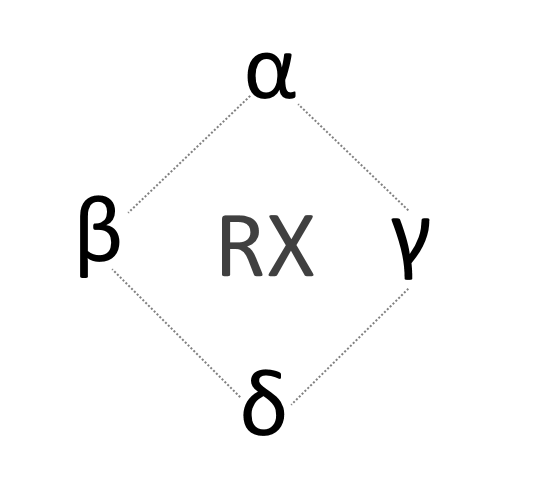
\includegraphics[scale=0.15]{abgrx.png}
}
\newtheorem{Def}{Определение}[section]
\newtheorem{Th}{Теорема}[section]
\newtheorem{Lm}{Лемма}[section] 
\newtheorem{Pb}{Задача}[section]
\newtheorem{Qu}{Признак}[section]
\newtheorem{St}{Утверждение}[section]
\newtheorem{Sl}{Следствие}[section]
\newtheorem{Zm}{Замечание}[section]
\newtheorem{Con}{Условие}[section]
\usepackage{relsize}
\newcommand{\vel}{\mathlarger{\mathlarger{\upsilon}}}
\newcommand{\der}[1]{\overset{\cdot}{#1}}
\newcommand{\dder}[1]{\overset{\cdot \cdot}{#1}}
\newcommand{\Lim}[2]{\lim\limits_{#1\to #2}}
\newcommand{\Ch}[1]{\overset{#1}{=}}
\newcommand{\p}[1]{#1^{\prime}}
\newcommand{\pp}[1]{#1^{\prime\prime}}
\newcommand{\ol}[1]{\overline{#1}}
\newcommand{\oll}[1]{\overline{\overline{#1}}}
\newcommand{\ov}[2]{\overset{#1}{#2}}
\newcommand{\un}[1]{\underline{#1}}
\newcommand{\gr}[2]{\includegraphics[scale=#1]{../pics/#2}}
\usepackage{comment}

\begin{document}
\maketitle
\vspace{4cm}
	
	\begin{myquote}
	\begin{center}
		\textbf{Аннотация}\\
		\textit{
			В этой статье полностью решён первый и второй пункты.\\
			Были доказаны некоторые леммы, позволяющие удобно работать с эквивалентностьюб максимальностью и кратчайшестью ломаных.
			Также были доказаны два условия того, что ломаная является кратчайшей.
		}
	\end{center}
	\end{myquote}	
	
	\pagebreak

	\tableofcontents	
	
	\pagebreak

\section*{Введение}

Рассмотрим множество ломаных на решётке $\mathds{Z}\times \mathds{Z}$ с началом в точке $(0, 0)$

\begin{enumerate}
	\item Ломаную можно представить как путь в $\{(x, y)\in\mathds{R}^2\mid x\in \mathds{Z} \text{ или } y\in\mathds{Z}\}$
	Введём специальные обозначения, для задания ломаной.
	\begin{enumerate}
		\item[] $a, A$ -- отрезки направленные вправо и влево
		\item[] $b, B$ -- вверх и вниз
		
		Для удобства будут также использоваться аналоги:
		\begin{itemize}
			\item $a^{-1} = A$
			\item $b^{-1} = B$
		\end{itemize}
	\end{enumerate}
	\item Общее количество таких отрезков будем называть длиной ломаной.
	\begin{enumerate}
		\item []Допускается случай ломаной с длиной 0 --- $\varepsilon$
	\end{enumerate}
	\item Ломаная замкнутая, если её конец совпадает с началом
	\item Ломаная простая, если у неё нет самопересечений по вершинам (допускается пересечение начала и конца -- случай замкнутой ломаной)
	\item За алфавит $S$ будем обозначать множество $S = \{a, b, a^{-1}, b^{-1}\} = \{a, b, A, B\}$ 	
\end{enumerate}

Введём 2 операции над ломаными:
\begin{enumerate}
	\item Вытягивание и затягивание -- добавление в любое место пути $l\in\{aA, Aa, bB, Bb\}$
	\item Перенос -- мы можем свободно перемещать в любое место пути определённые комбинации. 
	
	В Теории групп есть понятие описывающие такие конструкции -- коммутатор.
	\begin{Def}
		Коммутатор -- для $f, g\in G$  $ [g, h] = ghg^{-1}h^{-1}$. 
	\end{Def}
\end{enumerate}

Говоря о теории групп, можно задать группу всех ломаных с учётом операций:

$G =\langle a, b\mid [x, y]z = z[x, y], x, y, z\in \{a, b, a^{-1}, b^{-1}\}\rangle\quad\quad $ (первая операция будет автоматически учтена, т.к. в группе произведение элемента и его обратного равно еденице (пустому слову в нашем случае))

\begin{Def}
	Обратное слово -- конкатенация обратных элементов в обратном порядке
\end{Def}

\begin{Zm}
	Если два слова эквивалентны, то произведение первого на обратное ко второму эквивалентно пустому слову. 
\end{Zm}
\begin{proof}
	$l\equiv m$
	
	$lm^{-1} \equiv ll^{-1}\equiv \varepsilon$
\end{proof}

\begin{Zm}
	Преобразования не изменяют  конечную точку
\end{Zm}
\begin{proof}
\begin{enumerate}
	\item мы добавляем движение в любую сторону и обратное к нему. Таким образом мы приходим в ту же точку
	\item ломаная двигается по квадрату, приходя в ту же точку
\end{enumerate}
\end{proof}
\section{Проверка на эквивалентность}

\begin{enumerate}
	\item $babAAba\equiv bbb\qquad $ $babA[AbaB]BB\equiv ba[AbaB]bABB = b[aA]ba[Bb]ABB\equiv bb[aA]BB \equiv b[bB]B \equiv bB\equiv \varepsilon\Rightarrow bbb \equiv bbabAAba$
	\item $bbA\not \equiv aaB$
	\begin{Zm}
	Никакое движение не изменяет чётность количества букв а и b (и заглавных и строчных)
	\begin{itemize}
		\item вставка $zZ, z\in \{a, b, A, B\}$ -- добавляет две одинаковые буквы. чётность не меняется
		\item по сути это просто перемещение определённой группы букв, что не меняет их количество.
	\end{itemize}
	\end{Zm}
	В этих словах разное по чётности количество букв $a$ и $b\Rightarrow$ они не эквивалентны
	\item $aabbAABB$ и $abAB$.
	 
\end{enumerate}

\begin{multicols}{2}
\gr {0.25} {babAAba} \gr{0.25} {bbb}\columnbreak

$babAAba$ и $bbb$. 
$babA[AbaB]BB\equiv ba[AbaB]bABB = b[aA]ba[Bb]ABB\equiv bb[aA]BB \equiv b[bB]B \equiv bB\equiv \varepsilon\Rightarrow bbb \equiv bbabAAba$
\end{multicols}

\begin{multicols}{2}
\gr{0.25}{bbA} \gr {0.25} {aaB}\columnbreak

$aabbAABB$ и $abAB$
\begin{Zm}
	Никакое движение не изменяет чётность количества букв а и b (и заглавных и строчных)
	\begin{itemize}
		\item вставка $zZ, z\in \{a, b, A, B\}$ -- добавляет две одинаковые буквы. чётность не меняется
		\item по сути это просто перемещение определённой группы букв, что не меняет их количество.
	\end{itemize}
	\end{Zm}
	В этих словах разное по чётности количество букв $a$ и $b\Rightarrow$ они не эквивалентны
\end{multicols}

\begin{multicols}{2}
\gr{0.25}{aabbAABB} \gr{0.25}{abAB}\columnbreak

$aabbAABB$ и $abAB$

\begin{Def}
	У отрезков ломаной есть направление. Будем считать, что если в многоугольнике стороны направлены против часовой стрелке, то площадь положительна. В противном случае считаем её отрицательной.
\end{Def}

\end{multicols}
\begin{Zm}
При действии движений, если рассматривать многоугольник составленный из точек ломаной в порядке букв в слове, то его ориентированная площадь не изменится. Такой многоугольник существует, когда ломаная замкнутая.
\end{Zm}
\begin{proof}
Итак рассмотрим оба движения:
\begin{enumerate}
	\item вытягивание создаст две новых точки, но не добавит площади, т.к. на графике появится новый отрезок.
	\item вытягивание аналогично уберёт такой отрезок.
	\item перетаскивание квадрата вдоль сторон не изменит площадь, ведь площадь этого квадрата прибавляется к площади остальной фигуры, а его перемещение не меняет остальные стороны. 
\end{enumerate}

Понятно, что у слова $aabbAABB$ -- площадь 4, а у $abAB$ -- 1. А значит они не могут быть эквивалентны.
\end{proof}


\section{Кратчайшие ломаные}
\begin{Def}
	Ломаная является кратчайшей, если с помощью наших движений её нельзя перевести в ломаную с меньшей длиной.
\end{Def}

\subsection{Проверка того, что слово кратчайшее}
Является ли $abABabAB$ кратчайшей? $abAB[abAB] \equiv a[abAB]bAB\equiv aabAAB$. Мы с помощью движений получили слово меньшей длины, следовательно изначальной слово не является кратчайшим.

\subsection{Максимальные ломаные}

\begin{Def}
	Префикс ломаной L --- любая ломаная, не превосходящая по длине ломаную L и идущая по тому же маршруту. 
\end{Def}

\begin{Def}
	Ломаная называется максимальной, если она является кратчайшей и единственная кратчайшая ломаная для которой она является префиксом --- она сама.
\end{Def}

\begin{Th}
	Конец ломаной сохраняется при движениях
\end{Th}
\begin{proof}
	\begin{enumerate}
		\item []
		\item Вытягивание/затягивание --- мы добавляем слово $xx^{-1}$, но оно замкнутое, т.е. мы возвращаемся в точку, из которой вышли.
		\item При переносе мы выделяем замкнутую ломаную и перемещаем её. При её перемещении  точка конца не меняется, т.к.'проходя' через это замкнутое слово мы также остаёмся той же точке, из которой мы начали.
	\end{enumerate}
\end{proof}

\begin{Th}
	У каждой ломаной есть единственное представление в виде $[a, b]^zb^ya^x$, где $[a, b] = aba^{-1}b^{-1}$, степень --- конкатенация, т.е. $[a, b]^2 = [a, b][a, b]$, а $\{x, y, z\}\in\mathds{Z}^3$
\end{Th}
\begin{proof}
	Сначала покажем, что такое представление в принципе есть:
	
	Если у нас есть слово $xy$, то мы можем 'переставить' их следующим образом : %TODO вставить таблицу перевода
	
	Таким образом мы можем переставить все $b$ вправо, а все $a$ влево. При этом накопится некоторое количество коммутаторов. С помощью действия 2 перемещаем их все влево и получаем форму $[a, b]^zb^ya^x$
	
	Теперь докажем, что она единственная. Допустим это не так, т.е. для какой-то ломаной есть два таких эквивалентных определения:
	
	$[a, b]^zb^ya^x\equiv [a, b]^{z_0}b^{y_0}a^{x_0}$ 
	
	Рассмотрим фактор группу $G/_{\{[a, b]^z|z\in \mathds{Z}\}}$ Понятно, что это фактор группа, ведь группа, указанная в индексе --- нормальная.
	
	В нём вышеописанные слова соответствуют следующим классам:
	
	$b^ya^x\equiv b^{y_0}a^{x_0}$
	
	Эти ломаные должны быть равны. А значит у них совпадают конечные точки. Т.е. $(x, y) = (x_0, y_0)\Rightarrow x = x_0, y = y_0$
	
	Теперь вернёмся обратно в $G:$
	
	$[a, b]^zb^ya^x\equiv [a, b]^{z_0}b^{y_0}a^{x_0}$
	
	$[a, b]^zb^ya^xa^{-x_0}b^{-y_0}[a, b]^{-z_0}\equiv \varepsilon$
	
	$[a, b]^{z-z_0}b^ya^{x-x_0}b^{-y_0}\equiv [a, b]^{z-z_0}b^{y-y_0} \varepsilon [a, b]^{z-z_0}\equiv \varepsilon$
	
	Каждый $[a, b]$ добавляет ориентированной площади одну единицу. Справа ломаная с нулевой площадью. Слева с площадью $z-z_0$. Т.к. при движениях площадь сохранятся, то $z-z_0 = 0\Rightarrow z=z_0$
	
	Теорема доказана
\end{proof}

\begin{Zm}
	Такая запись показывает, что конечная точка ломаной --- $(x, y)$, и если она замкнутая, то $z$ --- её площадь.
	
	Эти характеристики будут сохраняться при движения, а значит будет разумно обозначить множества таких эквивалентных слов за класс $(z, y, x)$: $[a, b]^zb^za^x$
\end{Zm}

\begin{Zm}
	$\{(z, y, x)| x, y, z \in \mathds{Z}\}$ --- группа, на которой можно задать операцию следующим образом:
	\begin{enumerate}
		\item[] $(z_1, y_1, x_1) * (z_2, y_2, x_2) = (z_1 + z_2 + x_1*y_2, y_1 + y_2, x_1 + x_2)$. Она определена таким образом, потому что при конкатенации двух слов можно перенести все коммутаторы, но для того, чтобы привести к универсальной записи, нужно переместить $y_2$ букв $b$ через $x_1$ букв $a$. А для этого нужно использовать $x_1*y_2$ коммутаторов.
	\end{enumerate}
\end{Zm}

Раз мы завели классы, то разумно будет завести некоторый набор конструкций для удобной работы с ними

\begin{Def}
	Длиной класса будем называть длину кратчайшей ломаной в этом классе. И будем обозначать, как $len((z, y, x))$
\end{Def}

\begin{Def}
	За $class(w)$ будет обозначать переход от представителя класса к классу
	
	$class(a^{x_0}) = (0, 0, x_0)\qquad (z, y, x) * (0, 0, x_0) = (z, y, x+x_0)$ У соседних '$a$-шек' степени просто складываются.
	
	$class(b^{y_0}) = (0, y_0, 0)\qquad (z, y, x) * (0, y_0, 0) = (z + x*y_0, y+y_0, x)$ $\quad y_0$ букв $b$ нужно 'провести' через $x$ букв $a$, что образует $x*y_0$ коммутаторов, которые при приведении к нормальному виду перенесутся влево и прибавятся к уже имеющимся.
	
	$class([a, b]^{z_0}) = (z_0, 0, 0)$
\end{Def}

\begin{Lm}
	Если у ломаной некратчайший префикс, то сама ломаная--- некратчайшая.
\end{Lm}
\begin{proof}
	Пусть $l$ --- ломаная с некратчайшая префиксом $w$. Тогда её можно представить следующим образом. $l = w * l_0$, где $l_0$ часть слова после префикса. Т.к. $w$ --- неркатчайшая ломаная, то существует $\p w: w\equiv \p w\& |\p w|<|w|$. А значит $l = w*l_0\equiv \p w*l_0 = \p l$ и $|l| = |w*l_0| = |w| + |l_0| < |\p w| + |l_0| = |\p w*l_0| = |\p l|$ Т.е. мы нашли слово $\p l$, которое эквивалентно $l$ и длина которого меньше длины $l$. А значит $\p l$ --- некратчайшая.
\end{proof}

\begin{Def}
	Класс $(z, y, z)$ будем называть максимальным, если $len((z, y, x)*class(s))<len((z, y, x)) , \forall s\in S$
	
	Это по сути означает, что в классе есть максимальная ломаная
\end{Def}
\begin{proof}
	Пусть в классе $(z, y, x)$ есть максимальная ломаная $l$. Тогда $l$ --- кратчайшая, а значит длина класса равна длине $l$. И, так как $l$ --- максимальная, то $l * s, s\in S$ --- некратчайшая. А значит $len((z, y, x)*class(s)) < |l*s| = |l|+1$. Т.е. $len((z, y, x)) = |l|\geqslant  len((z, y, x)*class(s))$
	
	Равенства длин не может быть. Допустим обратное. Не умаляя общности скажем, что $|l|$ --- чётная. В противном случае можно будет провести аналогичные рассуждения. $|l * s|$ --- нечётная. мы знаем, что движения не изменяют чётность количества каждой из букв, а значит и чётность длины всего слова. Т.е. не существует движения, которое перевело бы слово с нечётной длиной к слову с чётной и наоборот, а значит $|l|$ и $|l*s|$ не могут быть равны.
	
	А значит $len((z, y, x)*class(s))<len((z, y, x))$
	
	В обратную сторону: Пусть $len((z, y, x)*class(s))<len((z, y, x)) , \forall s\in S$. Пусть в $(z, y, x)$ нет кратчайших ломаных. \\Тогда возьмём любую кратчайшую ломаную $l\in (z, y, x)$. $|l*s| < |l|~~ \forall s\in S$
	
	Нам нужно доказать, что нет кратчайшей ломаной (не равной $l$), такой что $l$ --- её префикс.
	
	Рассмотрим такую ломаную. Её можно представить, как $l * w, w\neq \varepsilon$ Так как $w\neq \varepsilon$, то можно выделить в $w$ первую букву $s$. Т.е. $l*w = l*s*\p w$. Но мы знаем, что $l*s$ --- некратчайшая. $l*s$ является префиксом слова $l*w$, а значит и оно некратчайшее. 
	
	Таким образом, мы доказали, что любое продолжение слова $l$ --- некратчайшее. При этом $l$ --- кратчайшее, а значит $l$ --- максимальное.
	
	
\end{proof}	

\begin{Lm}
	$ws$ -- не кратчайшее, $w$ -- кратчайшее. $v$ -- кратчайшее и $v\equiv ws$
\end{Lm}

\begin{Th}
	Для кратчайшей ломаной $l$ и буквы $s$ выполнятся следующее 
	
	$ls$ -- кратчайшая ломаная $\Longleftrightarrow$ в классе $[w]$ нет кратчайшего представителя, оканчивающегося на $s^{-1}$ 
\end{Th}
\begin{proof}
	Пусть $ls$ -- кратчайшая ломаная. Пусть существует $\p l s^{-1}\equiv w$. Тогда $[ls] = [\p l s s^{-1}] = [\p l]$, где $\p l$  -- префикс $l$ и $|l| = |\p l| + 1$.
	
	$|ls| = |l| + 1 = |\p l| + 2$. Но получается, что в классе $[ls]$ существует слово с меньшей длиной, чем $ls$ и при этом $ls$ -- кратчайшая. Противоречие
	
	Теперь в обратную сторону: Пусть а классе $(z, y, x)$ нет кратчайшего представителя, оканчивающегося на $s^{-1}$. И пусть $ls$ -- не кратчайшее. Пусть $[ls] = [\p l]$, где $\p l$ -- кратчайшее
\end{proof}

\begin{Th}
	Класс ломаных максимален $\Longleftrightarrow$ в этом классе есть кратчайшие слова, оканчивающиеся на все буквы алфавита $S$
\end{Th}
\begin{proof}
	Пусть в классе $(z, y, x)$ есть кратчайшие слова, оканчивающиеся на все буквы алфавита $S$. 
\end{proof}

\begin{Th}
	Любая кратчайшая замкнутая ломаная --- максимальная.
\end{Th}
\begin{proof}
	Итак, рассмотрим кратчайшую замкнутую ломаную $l$. Раз она замкнутая, то её конечная точка --- точка $(0, 0)$, а значит она принадлежит классу $(z, 0, 0)$. 	
	
	А тогда все такие слова лежат в классе коммутатора в какой-то степени $z$.
	
	А у для коммутаторов выполняется следующее равенство $[a, b] \equiv [ba^{-1}] \equiv [b^{-1}a]\equiv [a^{-1}b^{-1}]$
	
	$[a, b] = aba^{-1}b^{-1}\equiv aba^{-1}b^{-1}a^{-1}a\equiv a^{-1}aba^{-1}b^{-1}a^{-1}\equiv ba^{-1}b^{-1}a = [b, a^{-1}]$
	
	аналогично доказывается для остальных
	
	Таким образом в этом классе есть слова, заканчивающиеся на любую букву. А тогда, по предыдущей теореме этот класс максимален. А тогда все кратчайшие ломаные в этом классе --- максимальные. А значит все кратчайшие замкнутые ломаные --- максимальные. Теорема доказана.	
\end{proof}

\subsection{Каждая кратчайшая ломаная простая?}

\begin{Th}
	Если ломаная кратчайшая, то она простая. 
\end{Th}
\begin{proof}
	Докажем эквивалентное условие: Любая непростая ломаная --- некратчайшая.
	
	Итак, пусть в ломаной $l$ есть самопересечение. Рассмотрим часть ломаной  $w$ от пересечения до пересечения:
	\begin{enumerate}
		\item $w$ --- некратчайшая ломаная, а тогда и $l$ --- некратчайшая
		\item $w$ --- кратчайшая замкнутая ломаная, т.е. максимальная ломаная. А значит она представима в виде $[a, b]^z, z\in \mathds{Z}\setminus \{0\}$. Тогда передвинем все эти коммутаторы на одну букву назад. Другими словами возьмём букву перед  $w$ и протащим её через $z$ коммутаторов. Получится, что на конце $l$ есть максимальная ломаная с приписанной буквой. По определению максимальной ломаной, такоке слово не будет кратчайшим. А значит на конце ломаной $l$ есть некратчайшая часть $\Rightarrow l$ --- некратчайшее
	\end{enumerate}
\end{proof}
\subsection{Достаточные условия кратчайшей ломаной}
\begin{Def}
Ломаную мы будем называть кратчайшей, если её нельзя с помощью вытягивания, затягивания
или переноса привести к ломаной, имеющей меньшую длину.
\end{Def}

\begin{Con}
	$L \text{--- кратчайшая}\Longleftrightarrow\nexists \p L: \p L\equiv L ~\&~ len(\p L)<len(L)$
\end{Con}
\begin{proof}
	Пусть $\exists \p L: \p L\equiv L ~\&~ len(\p L)<len(L)$, а тогда мы можем движениями (вытягиваниями, затягиваниями и переносами) привести ломаную $L$  к ломаной $\p L$, что противоречит определению кратчайшести.
\end{proof}	

\begin{Con}
	Ломаная кратчайшая, когда она является частью кратчайшей ломаной
\end{Con}
\begin{proof}
	Допустим противное: пусть ломаная $L$ является частью кратчайшей ломаной $M$ и при этом сама $L$ не является кратчайшей. Тогда существует ломаная $\p L: \p L\equiv L~\&~ len(\p L)<len(L)$
	
	А значит, что ломаную $L$ можно движениями привести к меньшей по длине ломаной $p L$. Но все те же самые движения можно провести внутри ломаной $M$. Представим ломаную $M$ как $m + L + \p m$, где $m$ и $\p m$ --- части ломаной до и после ломаной $L$, а '+' означает конкатенацию. 
	
	Т.к. $L\equiv \p L$, то $m + L + \p m\equiv m+\p L + \p m$. Длина ломаной при конкатенации считается, как сумма длин её частей. Получается, что $len(M) = len(m+L+\p m) = len(m) + len(L) + len(\p m) < len(m) + len(\p L) + len(\p m) = len(m+\p L + \p m)$ и при этом $m+L+\p m\equiv m+\p L+\p m$. Но это противоречит условию, что $M$ --- кратчайшая?!
	
	
\end{proof}

\section{Замкнутые кратчайшие ломаные}

\section{Описание всех максимальных ломаных}
\begin{Th}
	Все максимальные ломаные --- кратчайшие замкнутые ломаные	
\end{Th}

\end{document}